\documentclass[10pt,aspectratio=169]{beamer}
\usetheme{Madrid}
\usecolortheme{default}
\usepackage{iftex}
\ifPDFTeX
  \usepackage[utf8]{inputenc}
  \usepackage[T2A]{fontenc}
\else
  \usepackage{fontspec}
  \setmainfont{Arial}
  \setsansfont{Arial}
\fi
\usepackage[russian]{babel}
\usepackage{amsmath}
\usepackage{booktabs}
\usepackage{graphicx}
\setbeamertemplate{navigation symbols}{}
\graphicspath{{images/}}
\title[Exclusive Self Attention]{Exclusive Self Attention}
\author[Иван Бобошко]{Иван Бобошко}
\date{26 октября 2026}
\begin{document}

\begin{frame}
\titlepage
\end{frame}

\begin{frame}[t]{Мотивация}
Attention собирает информацию не только из предыдущих токенов, но и из самого текущего токена:
\[
y_i=
\underbrace{\sum_{j<i}a_{ij}v_j}_{\text{контекст}}
+\underbrace{a_{ii}v_i}_{\text{собственный вклад}},
\qquad v_i=W_Vx_i.
\]
\vspace{0.2cm}
MLP уже выполняет pointwise-преобразование: обрабатывает каждую позицию независимо, не смешивая токены.
\[
\mathbb{FFN}(h_i)=W_2\,\sigma(W_1h_i+b_1)+b_2.
\]

\vspace{0.3cm}
Гипотеза: cобственный вклад в attention частично дублирует работу FFN. Attention тратит свои ёмкость на pointwise-признаки, конкурирующие с моделированием контекста.
\end{frame}

\begin{frame}[t]{Attention similarity bias}
Attention similarity bias -- это склонность выхода attention $y_i$ быть направленным вдоль собственного value-вектора $v_i$:
\begin{center}
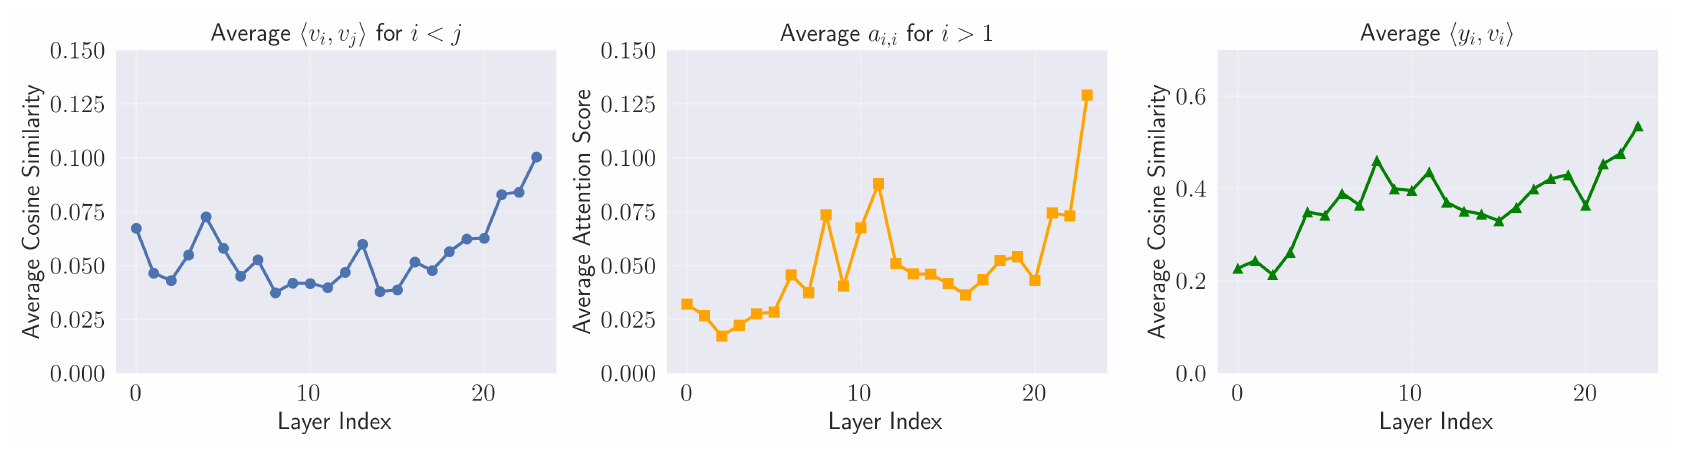
\includegraphics[width=\textwidth,height=0.44\textheight,keepaspectratio]{attention_similarity_bias_paper.png}
\end{center}

\vspace{0.25cm}
{ Слева: сходство разных $v_i,v_j$. В центре: вес $a_{ii}$. Справа: сходство $y_i,v_i$.}

\end{frame}

\begin{frame}[t]{Почему недостаточно просто удалить $v_i$}
Корреляция value векторов
\[
\begin{aligned}
v_j &= \alpha_jv_i+v_j^{\perp},\\[0.15cm]
\sum_{j<i}a_{ij}v_j
&=\left(\sum_{j<i}a_{ij}\alpha_j\right)v_i
+\sum_{j<i}a_{ij}v_j^{\perp}.
\end{aligned}
\]
Даже без собственного слагаемого выход может быть направлен вдоль $v_i$.
\vspace{0.3cm}

Диагональный вес как attention sink
\begin{itemize}
\setlength{\itemsep}{0.3cm}
\item Маскирование диагонали заставляет распределить всю массу по предыдущим токенам, даже если контекст не нужен.
\item XSA сохраняет $a_{ii}$: часть массы можно направить в собственный вклад, который затем удаляется проекцией.
\end{itemize}
\end{frame}

\begin{frame}[t,fragile]{Метод}
Сначала считаем обычный attention:
\[
y_i=\sum_{j\leq i}a_{ij}v_j.
\]
Затем вычитаем компоненту вдоль собственного value-вектора:
\[
\hat v_i=\frac{v_i}{\|v_i\|_2},
\qquad
z_i=y_i-\underbrace{(y_i^\top\hat v_i)\hat v_i}_{\text{проекция на направление }v_i},
\qquad z_i^\top v_i=0.
\]
\vspace{0.2cm}
\textbf{Две строчки}
\begin{verbatim}
v_unit = F.normalize(v, dim=-1)
z = y - (y * v_unit).sum(dim=-1, keepdim=True) * v_unit
\end{verbatim}
\end{frame}

% Shuangfei Zhai, Exclusive Self Attention, Figure 3, arXiv:2603.09078, CC BY 4.0.
\begin{frame}{Результаты}
\centering
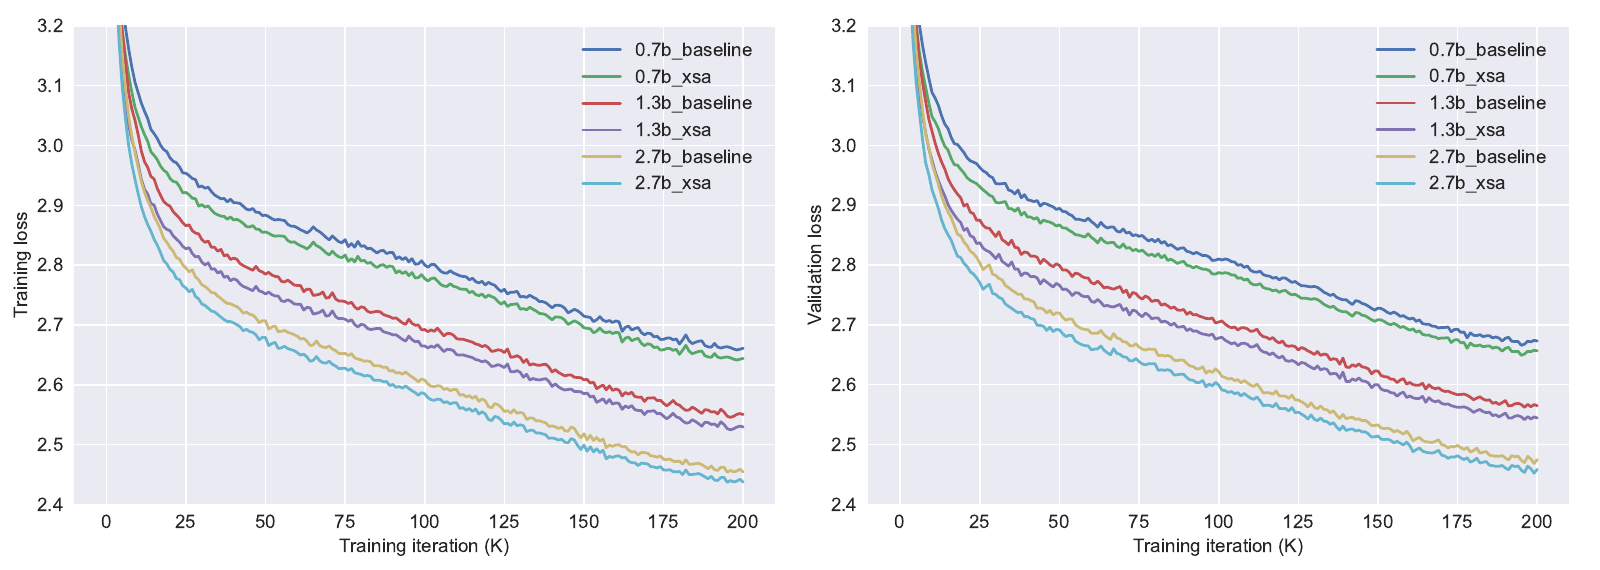
\includegraphics[width=\textwidth,height=0.68\textheight,keepaspectratio]{results_paper.png}

\vspace{0.3cm}
В экспериментах статьи XSA даёт более низкий train и validation loss, чем SA.
\end{frame}

% Shuangfei Zhai, Exclusive Self Attention, Figures 4 and 5 (validation panels), CC BY 4.0.
\begin{frame}{Другие эксперименты}
\begin{columns}[T,onlytextwidth]
\begin{column}{0.48\textwidth}
\centering
\textbf{Learning rate}

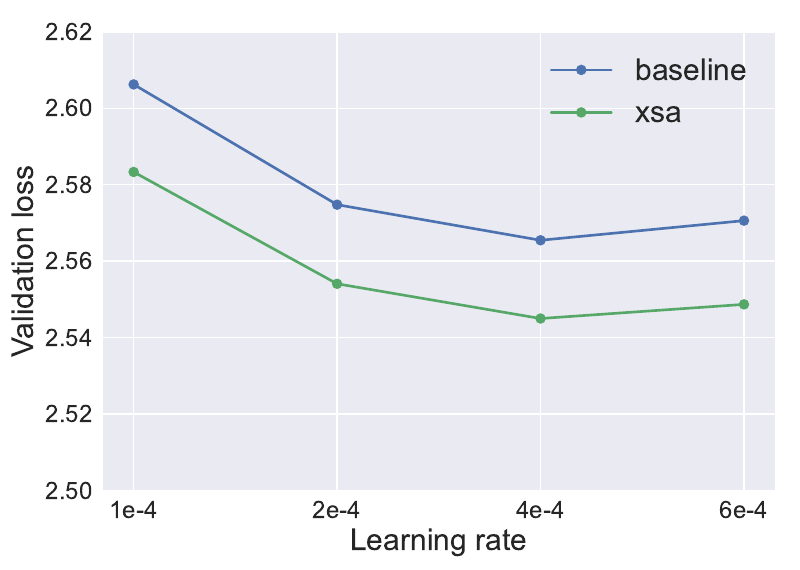
\includegraphics[width=\linewidth,height=0.48\textheight,keepaspectratio]{lr_paper_val.png}

XSA лучше SA при всех проверенных learning rate.
\end{column}
\begin{column}{0.48\textwidth}
\centering
\textbf{Длина контекста}

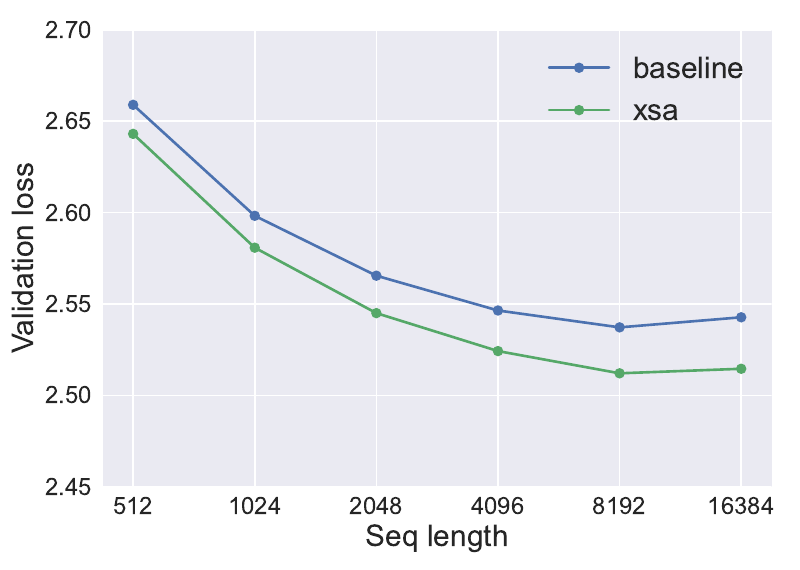
\includegraphics[width=\linewidth,height=0.48\textheight,keepaspectratio]{context_paper_val.png}

Выигрыш XSA в целом растёт с увеличением контекста.
\end{column}
\end{columns}
\vspace{0.3cm}
\small Модель 1.3B, validation loss. При изменении контекста число токенов на шаг фиксировано. Графики из Figures 4 и 5 статьи.
\end{frame}

\begin{frame}[t]{Список литературы}
\textbf{Статья}

Shuangfei Zhai. \emph{Exclusive Self Attention}, 2026.

\href{https://arxiv.org/abs/2603.09078}{\texttt{arxiv.org/abs/2603.09078}}

\vspace{0.6cm}
\textbf{Видео}

\href{https://youtu.be/2eZKT4H9_iQ?si=jv96E0irovFDeGmD}{\texttt{youtu.be/2eZKT4H9\_iQ}}
\end{frame}

\end{document}
